\documentclass{article}
\usepackage{amsmath}
\usepackage{tikz}
\usepackage{pgfplots}
\usepackage{setspace}
\usepackage{color}
\usetikzlibrary{positioning,quotes}
\usepackage[letterpaper,total={6in, 8in}]{geometry}

\usepgfplotslibrary{fillbetween}
\pgfplotsset{compat=1.18}
\title{Devoir 2}
\author{Emeric Laberge, Arpad Botond Rigo}
\date{\today}
\begin{document}
\begin{titlepage}
   \begin{center}
      \vspace*{1cm}
                  
      \Huge
      \textbf{Devoir 2}
                  
      \vspace{0.5cm}
      \LARGE
                  
      \vspace{1.5cm}
                  
      \textbf{Emeric Laberge\\Arpad Botond Rigo}
                  
      \vfill
                  
      Dans le cadre du cours\\
      IFT 1575
      
                  
      \vspace{0.8cm}
                  
      
\includegraphics[width=0.4\textwidth]{Université-de-Montréal.jpg}
                   
      \Large
      Département d'informatique et de recherche opérationnelle\\
      Université de Montréal\\
      Canada\\
      21 février 2023
                  
 	\end{center}
\end{titlepage}
\section*{Question 1}
\begin{equation*}
   \begin{aligned}
      & \underset{}{\text{minimiser}}
      & & z = -2x_1 - 3x_2 \\
      & \text{sujet à}
      & & x_1 + 3x_2 \le 6 \\
        &   &   & 3x_1 + 2x_2 \le 6 \\
        &   &   & x_1, x_2 \ge 0    
   \end{aligned}
\end{equation*}
\subsubsection*{(a)}

\begin{equation*}
   \begin{aligned}
      & \underset{}{\text{minimiser}}
      & & z = -2x_1 - 3x_2 \\
      & \text{sujet à}
      & & x_1 + 3x_2 + x_3 = 6 \\
        &   &   & 3x_1 + 2x_2 + x_4 = 6    \\
        &   &   & x_1, x_2 , x_3,x_4 \ge 0 
   \end{aligned}
\end{equation*}

\begin{center}
   \begin{equation*}
      \begin{array}{|c|ccccc|c|}
         \hline
         \text{v.d} & x_1 & x_2 & x_3 & x_4 & -z & \text{t.d} \\ \hline
         x_3        & 1   & 3   & 1   &     &    & 6          \\ 
         x_4        & 3   & 2   &     & 1   &    & 6          \\ \hline 
         -z         & -2  & -3  &     &     & 1  & 0          \\ \hline
      \end{array}
   \end{equation*}
   Le point (0,0) donne un z de 0
   
   \begin{equation*}
      \begin{array}{|c|ccccc|c|}
         \hline
         \text{v.d} & x_1 & x_2 & x_3  & x_4 & -z & \text{t.d} \\ \hline
         x_1        & 1/3 & 1   & 1/3  &     &    & 2          \\ 
         x_4        & 7/3 &     & -2/3 & 1   &    & 2          \\ \hline 
         -z         & -1  &     & 1    &     & 1  & 6          \\ \hline
      \end{array}
   \end{equation*}
   Le point (0,2) donne un z de -6
      
   \begin{equation*}
      \begin{array}{|c|ccccc|c|}
         \hline
         \text{v.d} & x_1 & x_2 & x_3  & x_4  & -z & \text{t.d} \\ \hline
         x_1        & 0   & 1   & 3/7  & -1/7 &    & 12/7       \\ 
         x_2        & 1   &     & -2/7 & 3/7  &    & 6/7        \\ \hline 
         -z         &     &     & 5/7  & 3/7  & 1  & 41/42      \\ \hline
      \end{array}
   \end{equation*}
   Le point $(\frac{6}{7},\frac{12}{7})$ donne un z de $\frac{-48}{7}$ \\ 
   \vspace{5mm} %5mm vertical space
   \textbf{Ceci est la solution optimale}
   
\end{center}
\pagebreak
\subsection*{(b)} 
\begin{equation*}
   \begin{aligned}
      & \underset{}{\text{minimiser}}
      & & z= -(45+\lambda)\: x_1 -(80+\lambda)\:x_2\\
      & \text{sujet à}
      & & 5x_1 +20x_2 \leq 400\\
        &   &   & 10x_1+15x_2 \leq 450 \\
        &   &   & x_1, x_2 \ge 0       
   \end{aligned}
\end{equation*}
\begin{center}
   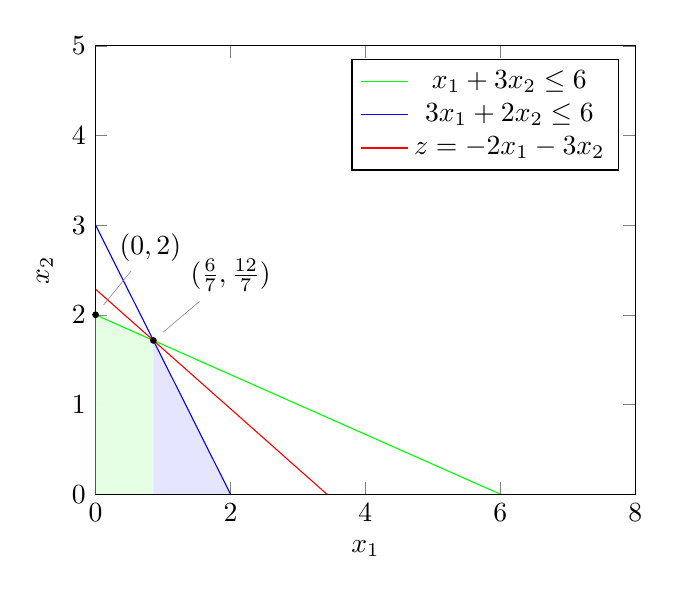
\begin{tikzpicture}
      \begin{axis}[
            xlabel=$x_1$,
            ylabel=$x_2$,
            ymin=0, ymax=5,
            xmin=0, xmax=8,
            legend pos=north east
         ]
         \addplot[color=green,name path=A,domain=0:85]{(6-x)/3};
         \addplot[color=blue,name path=B, domain=0:85]{(6-3*x)/2};
         \addplot[color=red,name path=D, domain=0:85]{(48/7-2*x)/3};
         \addplot[name path=C, domain=0:85]{0};
         \addplot[green!10, opacity=0.99] fill between[of=A and C, soft clip={domain=0:6/7}];
         \addplot[blue!10, opacity=0.99] fill between[of=B and C, soft clip={domain=6/7:2}];
         \addplot[mark=* , mark size = 1,color=black] coordinates {(6/7,12/7)} node[pin=55:{$(\frac{6}{7},\frac{12}{7})$}]{};
         \addplot[mark=* , mark size = 1,color=black] coordinates {(0,2)} node[pin=72:{$(0,2)$}]{};
      
                           
                           
                           
         \addlegendentry{$x_1 + 3x_2 \le 6$}
         \addlegendentry{$3x_1 + 2x_2 \le 6 $}
         \addlegendentry{$z = -2x_1 - 3x_2$}
                           
      \end{axis}
   \end{tikzpicture}
\end{center}

\pagebreak
% subsubsection a (end)
\section*{Question 2}
\subsubsection*{(a)}
\begin{equation*}
   \begin{aligned}
      & \underset{}{\text{minimiser}}
      & & z= -(45+\lambda)\: x_1 -(80+\lambda)\:x_2\\
      & \text{sujet à}
      & & 5x_1 +20x_2 \leq 400\\
        &   &   & 10x_1+15x_2 \leq 450 \\
        &   &   & x_1, x_2 \ge 0       
   \end{aligned}
\end{equation*}
\begin{center}
   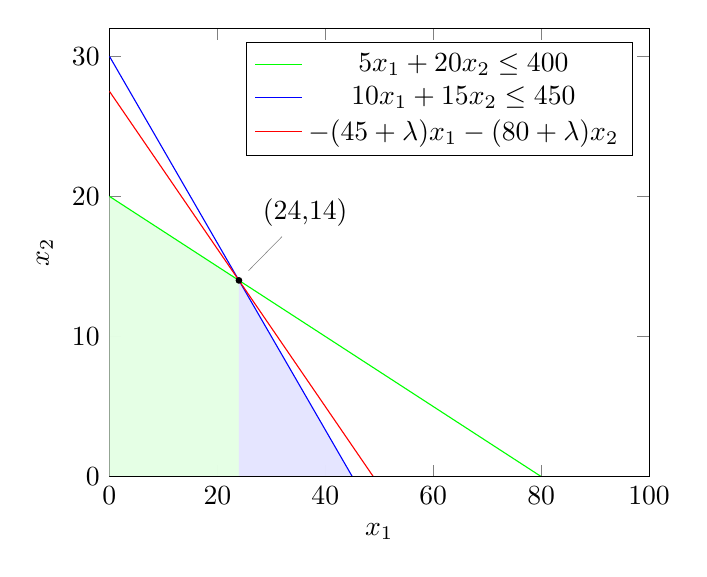
\begin{tikzpicture}
      \begin{axis}[
            xlabel=$x_1$,
            ylabel=$x_2$,
            ymin=0, ymax=32,
            xmin=0, xmax=100,
            legend pos=north east
         ]
                           
         \addplot[color=green,name path=A,domain=0:85]{(400-5*x)/20};
         \addplot[color=blue,name path=B, domain=0:85]{(450-10*x)/15};
         \addplot[color=red,name path=D, domain=0:85]{(2200-45*x)/80};
         \addplot[name path=C, domain=0:85]{0};
         \addplot[green!10, opacity=0.99] fill between[of=A and C, soft clip={domain=0:24}];
         \addplot[blue!10, opacity=0.99] fill between[of=B and C, soft clip={domain=24:45}];
         \addplot[mark=* , mark size = 1,color=black] coordinates {(24,14)} node[pin=72:{(24,14)}]{};

         \addlegendentry{$5x_1 +20x_2 \leq 400$}
         \addlegendentry{$10x_1+15x_2 \leq 450$}
         \addlegendentry{$-(45+\lambda)x_1-(80+\lambda)x_2$}
                           
      \end{axis}
   \end{tikzpicture}
\end{center}
\pagebreak
\subsection*{(b)}
Pour avoir la même solution optimale, on voit que la condition à respecter est que la pente de la droite à minimiser doit être supérieure à celle de la droite bleue ($5x_1 +20x_2 \leq 400$) et inférieure à celle de la droite verte ($10x_1+15x_2 \leq 450$).\\
Nous pouvons donc résoudre deux systèmes d'inéquations pour avoir la borne inférieure et la borne supérieure de la variable $\lambda$
\begin{spacing}{2.5}
   \begin{align*}
      \begin{matrix}
      \begin{aligned}
      \frac{-(45 + \lambda)x_1}{80 + \lambda} & < \frac{-5x_1}{20}                        \\
      \frac{45+\lambda}{80+\lambda}        & > \frac{1}{4}                            \\
      45+\lambda                           & > \frac{1}{4}(80+\lambda)                \\
      45+\lambda                             & > 20+\frac{\lambda}{4}                   \\
      \frac{3\lambda}{4}                     & > -25                                       \\
      \lambda                                 & > \frac{-100}{3}                          
      \end{aligned}
                                              &                                           
      \begin{aligned}
      \frac{-10x_1}{15}                       & < \frac{-(45 + \lambda)x_1}{80 + \lambda} \\
      \frac{2}{3}                            & > \frac{45+\lambda}{80+\lambda}        \\
      \frac{2}{3}(80+\lambda)                & > 45+\lambda                           \\
      \frac{160}{3} + \frac{2\lambda}{3}    & > 45+\lambda                             \\
      \frac{25}{3}                           & > \frac{\lambda}{3}                      \\
      25                                      & >\lambda                                  
      \end{aligned}
      \end{matrix}
   \end{align*}
\end{spacing}
\textbf{Nous avons donc que $\lambda = [\frac{-100}{3} , 25]$}
\pagebreak
\section*{Question 3}
\subsection*{(a)}
\begin{center}
\begin{equation*}
   \begin{aligned}
      & \underset{}{\text{minimiser}}
      & & \sum_{\substack{j=1\\j\neq k}}^{n} c_jx_j+c_ku_k-c_kv_k\\
      & \text{sujet à}
         & & \sum_{\substack{j=1\\j\neq k}}^{n} a_{ij}x_j+a_{ik}u_k-a_{ik}v_k
         =b_i , \: i=1,...,m\\ 
        &   &   & x_j \geq 0,\quad 1,...,n ,\: j\neq k \\
        &   &   & u_k, v_k \ge 0       
\end{aligned}
\end{equation*}
\end{center}
\begin{spacing}{1.2}
\noindent Le modèle résolu, on obtient la solution optimale
$x_j^* , j = 1, ..., n, j \neq k, u^*_k, v^*_k, \text{avec }
x^*_k = u^*_k-v^*_k$
Si $a_{ik} = 0$ i=1, ..., m et si $c_k \neq 0$, alors la valeur de $a_{ik}$ étant de 0 fait en sorte que la valeur de $u_k$ et $v_k$ n'ont aucune influence sur le respect des contraintes.\\

\noindent Cela étant dit , nous savons également la valeur de  coefficient  de $c_k \neq 0$ et donc , nous pouvons ``pomper'' au maximum $u_k$ et faire en sorte  que $v_k=0$ dans le cas où $c_k < 0$.Inversement nous pouvons ``pomper'' au maximum $v_k$ et faire en sorte  que $u_k=0$ dans le cas où $c_k>0$\\

\noindent Le but de la manoeuvre étant que malgré le fait que ceci n'ait aucun impact sur les contraintes , l'effet sur l'objectif est tel que il est impossible de borner inférieurement le problème car plus on augmente $u_k$ ou $v_k$ dans les cas respectifs , plus on minimise l'objectif.\\

\noindent Sachant que $u_k$ et $v_k$ ne sont pas borné supérieurement , la réponse optimale implique d'avoir un coefficient infini à un des deux coefficients et donc le problème n'est pas borné inférieurement car on peut toujours plus minimiser.
\end{spacing}
\subsection*{(b)}
\begin{spacing}{1.2}
\noindent Considérant à nouveau la situation évoquée au point (a) où $a_{ik} = 0$, i = 1, ..., m et $c_k \neq 0$, la conclusion demeure-t-elle la même si on ajoute la contrainte $x_k \geq 0$? 
\\

\noindent En rajoutant la contrainte $x_k \geq 0$ on se retrouve borner inférieurement le problème dans le cas où $c_k > 0$, car dans ce cas, la solution en (a) ne va pas respecter $x_k \geq 0$ néanmoins , dans le cas où $c_k < 0$, le problème n'est pas borné inférieurement car la solution en (a) respecte la condition $x^*_k = u^*_k-v^*_k \geq 0$ et cette solution n'est pas bornée inférieurement.
\end{spacing}

\pagebreak

\section*{Question 4}
\subsection*{(a)} 
\begin{center}
   \begin{equation*}
      \begin{array}{|c|ccccccc|c|}
         \hline
         \text{v.d} & x_1 & x_2 & x_3 & x_4 & x_5 & x_6 & -z & \text{t.d} \\ \hline
         x_5        &  1  &  2  &  1  &  1  &     &     &    & 43  \\ 
         x_6        &  3  &     &  2  &     &  1  &     &    & 46 \\ 
         x_7        &  1  &  4  &     &     &     &  1  &    & 42 \\ \hline 
         -z         & -3  & -2  & -5  &     &     &     &  1 & 0 \\ \hline
      \end{array}
   \end{equation*}
   \vspace{5mm} %5mm vertical space
   $x_b=
   \begin{pmatrix}
     x_2\\
     x_3\\
     x_6\\
   \end{pmatrix}
   \:
   x_R =
   \begin{pmatrix}
     x_1\\
     x_4\\
     x_5\\
   \end{pmatrix}
   c_B =
   \begin{pmatrix}
     -2\\
     -5\\
     0\\
   \end{pmatrix}
   c_R =
   \begin{pmatrix}
     -3\\
     0\\
     0\\
   \end{pmatrix}
   b =
   \begin{pmatrix}
     43\\
     46\\
     42\\
   \end{pmatrix}
   A =
   \begin{pmatrix}
     1  &  2  &  1  &  1  &  0  &   0  \\
     3  &  0  &  2  &  0  &  1  &   0  \\  
     1  &  4  &  0  &  0  &  0  &  1  
   \end{pmatrix}$

   $ B =
   \begin{pmatrix}
      2 & 1 & 0\\
      0 & 2 & 0\\ 
      4 & 0 & 1
   \end{pmatrix}$
   $ R =
   \begin{pmatrix}
     1  &  1  &  0 \\
     3  &  0  &  1 \\  
     1  &  0  &  0   
   \end{pmatrix}$
   $ B^{-1} =
   \begin{pmatrix}
      1/2 & -1/4 & 0\\
      0   & 1/2  & 0\\ 
      -2  & 1    & 1
   \end{pmatrix}$
   \\
   \vspace{5mm} %5mm vertical space
   $B^{-1}A=
   \begin{pmatrix}
      1/2 & -1/4 & 0\\
      0   & 1/2  & 0\\ 
      -2  & 1    & 1
   \end{pmatrix}
   \begin{pmatrix}
     1  &  2  &  1  &  1  &  0  &   0  \\
     3  &  0  &  2  &  0  &  1  &   0  \\  
     1  &  4  &  0  &  0  &  0  &  1  
   \end{pmatrix}
   = 
   \begin{pmatrix}
     -1/4  &  1  &  0  &  1/2  &  -1/4  &   0  \\
     3/2   &  0  &  1  &  0    &   1/2  &   0  \\  
     2     &  0  &  0  &  -2    &  1     &  1  
   \end{pmatrix}$
   \\
   \vspace{5mm} %5mm vertical space
   
   $B^{-1}b=
   \begin{pmatrix}
      1/2 & -1/4 & 0\\
      0   & 1/2  & 0\\ 
      -2  & 1    & 1
   \end{pmatrix}
   \begin{pmatrix}
     43\\
     46\\
     42\\
   \end{pmatrix}
   =
   \begin{pmatrix}
     10\\
     23\\
     2\\
   \end{pmatrix}$
   \\
   \vspace{5mm} %5mm vertical space
   $\pi^T=c^T_B B^{-1}=
   \begin{pmatrix}
      -2,&-5,&0
   \end{pmatrix}
   \begin{pmatrix}
      1/2 & -1/4 & 0\\
      0   & 1/2  & 0\\ 
      -2  & 1    & 1
   \end{pmatrix}
   =
   \begin{pmatrix}
      -1,&-2,&0
   \end{pmatrix}
   $
   \\
   \vspace{5mm} %5mm vertical space

   $c^T-\pi^TA=
   \begin{pmatrix}
      -3,&-2,&-5,&0,&0,&0
   \end{pmatrix}
   -
   \begin{pmatrix}
      -1,&-2,&0
   \end{pmatrix}
   \begin{pmatrix}
     1  &  2  &  1  &  1  &  0  &   0  \\
     3  &  0  &  2  &  0  &  1  &   0  \\  
     1  &  4  &  0  &  0  &  0  &  1  
   \end{pmatrix}
   $
   \\
   \vspace{5mm} %5mm vertical space

   $c^T-\pi^TA=
   \begin{pmatrix}
      -3,&-2,&-5,&0,&0,&0
   \end{pmatrix}
   -
   \begin{pmatrix}
      -7,&-2,&-5,&-1,&-2,&0
   \end{pmatrix}
   $
   \\
   \vspace{5mm} %5mm vertical space
   $c^T-\pi^TA=
   \begin{pmatrix}
      4,&0,&0,&1,&2,&0
   \end{pmatrix}$
   \\
   \vspace{5mm} %5mm vertical space
   
   $-\pi^Tb=
   \begin{pmatrix}
      1,&2,&0
   \end{pmatrix}
   \begin{pmatrix}
     43\\
     46\\
     42\\
   \end{pmatrix}
   =135$
\begin{spacing}{2}
   \begin{equation*}
      \begin{array}{|c|cc|c|}
         \hline
         \text{v.d} & x_1...x_n& -z & \text{t.d} \\ \hline

         x_B        & B^{-1}A&    & B^{-1}b \\ \hline 
         -z         &c^T-\pi^TA&  1 & -\pi^Tb\\ \hline
      \end{array}
   \end{equation*}
   \begin{equation*}
      \begin{array}{|c|ccccccc|c|}
         \hline
         \text{v.d} & x_1 & x_2 & x_3 & x_4 & x_5 & x_6 & -z & \text{t.d} \\ \hline
       x_2&  -1/4  &  1  &     &  1/2  &  -1/4  &   &   & 10 \\
       x_3&  3/2   &     &  1  &      &   1/2  &   &   & 23\\  
       x_6&  2     &     &     &  -2   &  1     & 1 &   & 2 \\ \hline 
       -z & 4    &   &    &  1   &  2     &  & 1 & 135 \\ \hline
      \end{array}
      \end{equation*}
\end{spacing}
\end{center}
\subsection*{(b)}
\begin{center}
$\tilde{b}=b+\Delta b
=
\begin{pmatrix}
     43\\
     46\\
     42\\
   \end{pmatrix}
   +
   \begin{pmatrix}
     \Delta\\
     0\\
     0\\
   \end{pmatrix}
    =
    \begin{pmatrix}
     43+\Delta\\
     46\\
     42\\
   \end{pmatrix}$
   \\ 
   \vspace{5mm} %5mm vertical space

   $\overline{\tilde{b}}=B^{-1}\tilde{b}
	=
	\begin{pmatrix}
      1/2 & -1/4 & 0\\
      0   & 1/2  & 0\\ 
      -2  & 1    & 1
   	\end{pmatrix}
    \begin{pmatrix}
     43+\Delta\\
     46\\
     42\\
   \end{pmatrix}
   =
   \begin{pmatrix}
     10+\Delta/2\\
     23\\
     2-2\Delta\\
   \end{pmatrix}$

\begin{spacing}{1.9}
   \begin{align*}
      \begin{matrix}
      \begin{aligned}
      10+ \frac{\Delta}{2} & \geq 0   \\
   		\frac{\Delta}{2} & \geq -10    \\
   		\Delta & \geq -20                     
      \end{aligned}
                                              &                                           
      \begin{aligned}
      2- 2\Delta & \geq 0   \\
   		-2\Delta & \geq -2    \\
   		\Delta & \leq 1                     
      \end{aligned}
      \end{matrix}
   \end{align*}
\end{spacing}

\textbf{L'interval de variation de $b_1$ est $-20\leq\Delta\leq 1$ et donc:}\\
$43-20\leq b_1+\Delta \leq 43 +1$\\
$23\leq b_1 \leq 44$\\
\textbf{$b_1=[23,44]$}  


\end{center}


\subsection*{(c)}
\begin{center}
$\overline{\tilde{b}}=B^{-1}\tilde{b}
	=
	\begin{pmatrix}
      1/2 & -1/4 & 0\\
      0   & 1/2  & 0\\ 
      -2  & 1    & 1
   	\end{pmatrix}
    \begin{pmatrix}
     44\\
     50\\
     41\\
   \end{pmatrix}
   =
   \begin{pmatrix}
     19/2\\ 
     25\\
     3\\
   \end{pmatrix}
   \geq 0$
   \\
   \vspace{5mm} %5mm vertical space

   La base reste donc optimale et nous avions déjà trouvé que $\pi^T = \begin{pmatrix}
      -1,&-2,&0
   \end{pmatrix}$ et donc : 
   \\
   \vspace{5mm} %5mm vertical space

   $\overline{\tilde{z}} = \pi^T\tilde{b} 
   =
   \begin{pmatrix}
      -1,&-2,&0
   \end{pmatrix}
   \begin{pmatrix}
     44\\ 
     50\\
     41\\
   \end{pmatrix}
   =
   -144$\\ 
   \vspace{5mm} %5mm vertical space
   La solution optimale est donc 
\begin{spacing}{1.5}
   \begin{equation*}
      \begin{array}{|c|ccccccc|c|}
         \hline
         \text{v.d} & x_1 & x_2 & x_3 & x_4 & x_5 & x_6 & -z & \text{t.d} \\ \hline
       x_2&  -1/4  &  1  &     &  1/2  &  -1/4  &   &   & 19/2 \\
       x_3&  3/2   &     &  1  &      &   1/2  &   &   & 25\\  
       x_6&  2     &     &     &  -2   &  1     & 1 &   & 3 \\ \hline 
       -z & 4    &   &    &  1   &  2     &  & 1 & 144 \\ \hline
      \end{array}
      \end{equation*}
\end{spacing}
\end{center}
\pagebreak
\subsection*{(d)}
\begin{spacing}{2}
\begin{equation*}
      \begin{array}{|c|ccccccc|c|}
         \hline
         \text{v.d} & x_1 & x_2 & x_3 & x_4 & x_5 & x_6 & -z & \text{t.d} \\ \hline
       x_2&  -1/4  &  1  &     &  1/2  &  -1/4  &   &   & 10 \\
       x_3&  3/2   &     &  1  &      &   1/2  &   &   & 23\\  
       x_6&  2     &     &     &  -2   &  1     & 1 &   & 2 \\ \hline 
       -z & 4    & \textcolor{red}{\Delta c_2} &    &  1   &  2     &  & 1 & 135 \\ \hline
      \end{array}
      \end{equation*}
\begin{equation*}
      \begin{array}{|c|ccccccc|c|}
         \hline
         \text{v.d} & x_1 & x_2 & x_3 & x_4 & x_5 & x_6 & -z & \text{t.d} \\ \hline
       x_2&  -1/4  &  1  &     &  1/2  &  -1/4  &   &   & 10 \\
       x_3&  3/2   &     &  1  &      &   1/2  &   &   & 23\\  
       x_6&  2     &     &     &  -2   &  1     & 1 &   & 2 \\ \hline 
       -z & 4 + \frac{\Delta c_2}{4}    &  &    &  1-\frac{\Delta c_2}{2}    &  2 + \frac{\Delta c_2}{4}      &  & 1 & 135 \\ \hline
      \end{array}
      \end{equation*}      
\begin{center}
   \begin{align*}
      \begin{matrix}
      \begin{aligned}
      4 + \frac{\Delta c_2}{4} & \geq 0   \\
       \frac{\Delta c_2}{4} & \geq -4   \\
		\Delta c_2 & \geq -16   \\                 
      \end{aligned}
                                              &                                           
      \begin{aligned}
      1-\frac{\Delta c_2}{2} & \geq 0   \\
      \frac{\Delta c_2}{2} & \leq 1   \\
      \Delta c_2 & \leq 2   \\
      \end{aligned}
                                              &                                           
      \begin{aligned}
      2+\frac{\Delta c_2}{4} & \geq 0   \\
      \frac{\Delta c_2}{4} & \geq -2   \\
      \Delta c_2 & \geq -8   \\
      \end{aligned}
      \end{matrix}
   \end{align*}
\end{center}
\end{spacing}
\begin{center}
\textbf{L'interval de variation de $c_2$ est $-8\leq\Delta c_2\leq2$ et donc:}\\
\textbf{$\Delta c_2=[-8,2]$}  

\end{center}



\pagebreak
\section*{Question 5}

\begin{equation*}
   \begin{aligned}
      & \underset{}{\text{minimiser}}
      & & z= -5x_1-4x_2 \\
      & \text{sujet à}
      & & x_1 +x_2 \leq 5\\
        &   &   & 10x_1 +6x_2 \leq 45               \\
        &   &   & x_1, x_2 \ge 0 \text{ et entier } 
   \end{aligned}
\end{equation*}
\begin{center}
   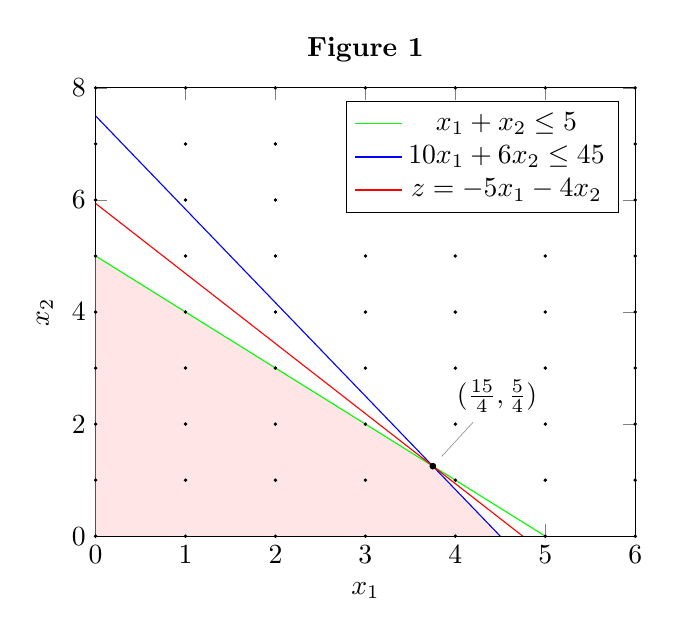
\begin{tikzpicture}
      \begin{axis}[
            xlabel=$x_1$,
            ylabel=$x_2$,
            title =\textbf{Figure 1},
            ymin=0, ymax=8,
            xmin=0, xmax=6,
            legend pos=north east
         ]
         \addplot[color=green,name path=A,domain=0:85]{(5-x};
         \addplot[color=blue,name path=B, domain=0:85]{(45-10*x)/6};
         \addplot[color=red,name path=D, domain=0:85]{(95/4-5*x)/4};
         \addplot[name path=C, domain=0:85]{0};
         \addplot[red!10, opacity=0.99] fill between[of=A and C, soft clip={domain=0:15/4}];
         \addplot[red!10, opacity=0.99] fill between[of=B and C, soft clip={domain=15/4:4.5}];
         \addplot[mark=* , mark size = 1,color=black] coordinates {(15/4,5/4)} node[pin=72:{$(\frac{15}{4},\frac{5}{4})$}]{};
         \foreach \a in {0,...,8}
         \foreach \b in {0,...,8}
         {\addplot[mark=* ,mark size = 0.4] coordinates {(\a,\b)};}
                     
                           
                           
         \addlegendentry{$x_1 +x_2 \leq 5$}
         \addlegendentry{$10x_1 +6x_2 \leq 45$}
         \addlegendentry{$z= -5x_1-4x_2$}
                           
      \end{axis}
   \end{tikzpicture}
   \\
   Le point trouvé est $(\frac{15}{4},\frac{5}{4})$ avec un z de valeur -23.75\\
   \textbf{En branchant sur la variable $x_2$, nous avons  $x_2 \leq 1$ et $x_2\geq 2$}
\end{center}
\pagebreak
\begin{equation*}
   \begin{aligned}
      & \underset{}{\text{minimiser}}
      & & z= -5x_1-4x_2 \\
      & \text{sujet à}
      & & x_1 +x_2 \leq 5\\
        &   &   & 10x_1 +6x_2 \leq 45               \\
        &   &   & x_2 \leq 1                        \\
        &   &   & x_1, x_2 \ge 0 \text{ et entier } 
   \end{aligned}
\end{equation*}
\begin{center}
   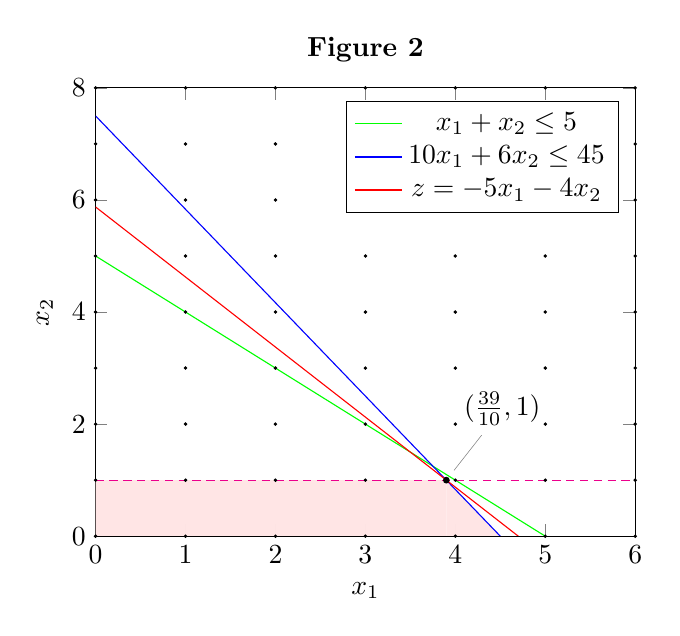
\begin{tikzpicture}
      \begin{axis}[
            xlabel=$x_1$,
            ylabel=$x_2$,
            title =\textbf{Figure 2},
            ymin=0, ymax=8,
            xmin=0, xmax=6,
            legend pos=north east
         ]
         \addplot[color=green,name path=A,domain=0:8]{(5-x};
         \addplot[color=blue,name path=B, domain=0:85]{(45-10*x)/6};
         \addplot[color=red,name path=D, domain=0:85]{(23.5-5*x)/4};
         \addplot[name path=C, domain=0:8 , transparent]{1};
         \addplot[name path=E, domain=0:8]{0};
         \addplot[red!10, opacity=0.99] fill between[of=E and C, soft clip={domain=0:3.9}];
         \addplot[red!10, opacity=0.99] fill between[of=B and E, soft clip={domain=3.9:4.5}];
         \addplot +[mark=none , color=magenta] coordinates {(0,1) (8, 1)};
         
         \addplot[mark=* , mark size = 1,color=black] coordinates {(39/10,1)} node[pin=80:{$(\frac{39}{10},1)$}]{};
         
         \foreach \a in {0,...,8}
         \foreach \b in {0,...,8}
         {\addplot[mark=* ,mark size = 0.4] coordinates {(\a,\b)};}
         
         
                           
                           
                           
         \addlegendentry{$x_1 +x_2 \leq 5$}
         \addlegendentry{$10x_1 +6x_2 \leq 45$}
         \addlegendentry{$z= -5x_1-4x_2$}
                           
      \end{axis}
   \end{tikzpicture}
   \\
   Le point trouvé est $(\frac{39}{10},1)$ avec un z de valeur -23.5\\
   Le point n'est pas entier donc nous introduisons $x_1\leq3$ et $x_1\geq4$
\end{center}

\pagebreak

\begin{equation*}
   \begin{aligned}
      & \underset{}{\text{minimiser}}
      & & z= -5x_1-4x_2 \\
      & \text{sujet à}
      & & x_1 +x_2 \leq 5\\
        &   &   & 10x_1 +6x_2 \leq 45               \\
        &   &   & x_2 \geq 2                        \\
        &   &   & x_1, x_2 \ge 0 \text{ et entier } 
   \end{aligned}
\end{equation*}
\begin{center}
   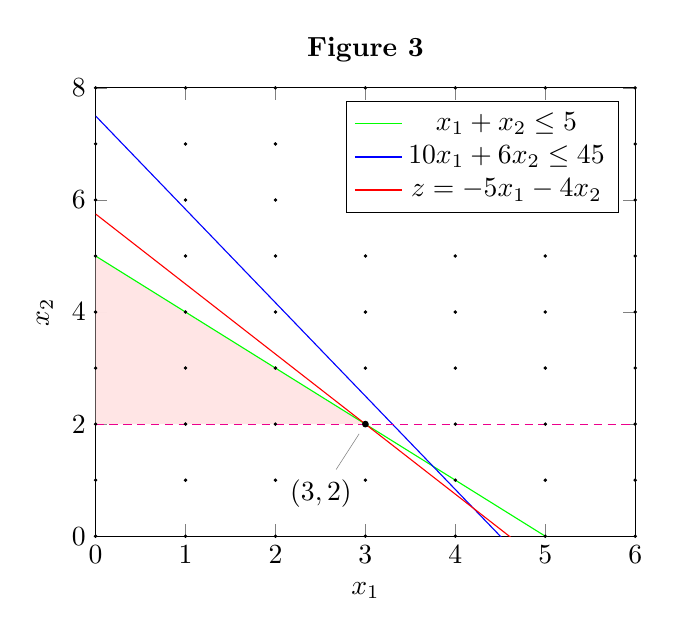
\begin{tikzpicture}
      \begin{axis}[
            xlabel=$x_1$,
            ylabel=$x_2$,
            title =\textbf{Figure 3},
            ymin=0, ymax=8,
            xmin=0, xmax=6,
            legend pos=north east
         ]
         \addplot[color=green,name path=A,domain=0:85]{(5-x};
         \addplot[color=blue,name path=B, domain=0:85]{(45-10*x)/6};
         \addplot[color=red,name path=D, domain=0:85]{(23-5*x)/4};
         \addplot[name path=C, domain=0:85,transparent]{2};
         \addplot[red!10, opacity=0.99] fill between[of=A and C, soft clip={domain=0:3}];
         \addplot +[mark=none , color=magenta] coordinates {(0,2) (8,2)};
         \addplot[mark=* , mark size = 1,color=black] coordinates {(3,2)} node[pin=265:{$(3,2)$}]{};
         
                  
         \foreach \a in {0,...,8}
         \foreach \b in {0,...,8}
         {\addplot[mark=* ,mark size = 0.4] coordinates {(\a,\b)};}
                           
                           
                           
         \addlegendentry{$x_1 +x_2 \leq 5$}
         \addlegendentry{$10x_1 +6x_2 \leq 45$}
         \addlegendentry{$z= -5x_1-4x_2$}
                           
      \end{axis}
   \end{tikzpicture}
   \\
   Le point trouvé est $(3,2)$ avec un z de valeur -23\\
   Le point est un entier donc nous ne branchons pas
   
      
\end{center}
\pagebreak
\begin{equation*}
   \begin{aligned}
      & \underset{}{\text{minimiser}}
      & & z= -5x_1-4x_2 \\
      & \text{sujet à}
      & & x_1 +x_2 \leq 5\\
        &   &   & 10x_1 +6x_2 \leq 45               \\
        &   &   & x_2 \leq 1                        \\
        &   &   & x_2 \leq 3                        \\
        &   &   & x_1, x_2 \ge 0 \text{ et entier } 
   \end{aligned}
\end{equation*}
\begin{center}
   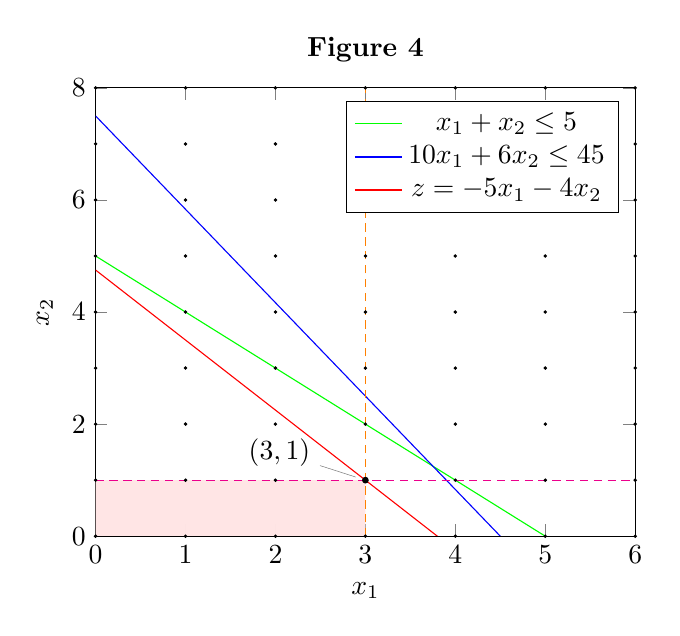
\begin{tikzpicture}
      \begin{axis}[
            xlabel=$x_1$,
            ylabel=$x_2$,
            title =\textbf{Figure 4},
            ymin=0, ymax=8,
            xmin=0, xmax=6,
            legend pos=north east
         ]
         \addplot[color=green,name path=A,domain=0:85]{(5-x};
         \addplot[color=blue,name path=B, domain=0:85]{(45-10*x)/6};
         \addplot[color=red,name path=D, domain=0:85]{(19-5*x)/4};
         \addplot[name path=C, domain=0:8 , transparent]{1};
         \addplot[name path=E, domain=0:8]{0};
         \addplot +[mark=none , color = orange] coordinates {(3,0) (3, 8)};
         \addplot +[mark=none , color=magenta] coordinates {(0,1) (8, 1)};
         
         \addplot[red!10, opacity=0.99] fill between[of=E and C, soft clip={domain=0:3}];
         
         \addplot[mark=* , mark size = 1,color=black] coordinates {(3,1)} node[pin=175:{$(3,1)$}]{};
         
         \foreach \a in {0,...,8}
         \foreach \b in {0,...,8}
         {\addplot[mark=* ,mark size = 0.4] coordinates {(\a,\b)};}
                           
                           
                           
         \addlegendentry{$x_1 +x_2 \leq 5$}
         \addlegendentry{$10x_1 +6x_2 \leq 45$}
         \addlegendentry{$z= -5x_1-4x_2$}
                           
      \end{axis}
   \end{tikzpicture}
   \\
   Le point trouvé est $(3,1)$ avec un z de valeur -19\\
   Le point est un entier donc nous ne branchons pas
\end{center}
\pagebreak

\begin{equation*}
   \begin{aligned}
      & \underset{}{\text{minimiser}}
      & & z= -5x_1-4x_2 \\
      & \text{sujet à}
      & & x_1 +x_2 \leq 5\\
        &   &   & 10x_1 +6x_2 \leq 45               \\
        &   &   & x_2 \leq 1                        \\
        &   &   & x_1 \geq 4                        \\
        &   &   & x_1, x_2 \ge 0 \text{ et entier } 
   \end{aligned}
\end{equation*}
\begin{center}
   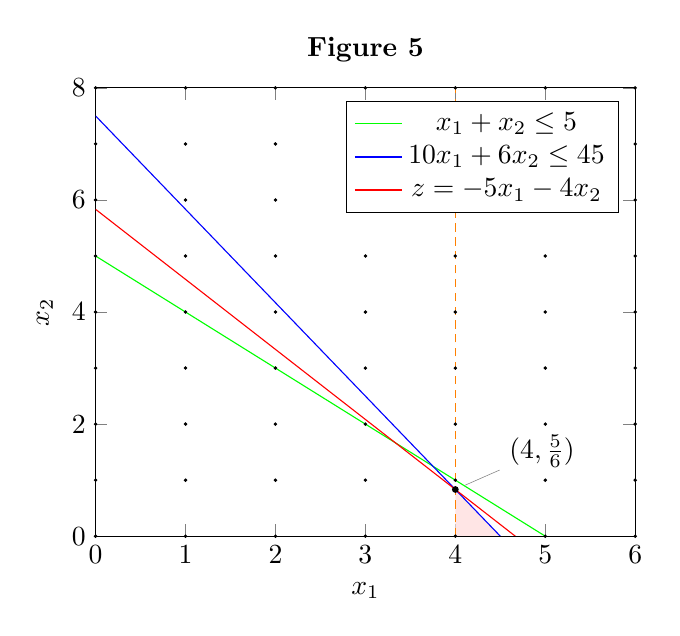
\begin{tikzpicture}
      \begin{axis}[
            xlabel=$x_1$,
            ylabel=$x_2$,
            title =\textbf{Figure 5},
            ymin=0, ymax=8,
            xmin=0, xmax=6,
            legend pos=north east
         ]
         \addplot[color=green,name path=A,domain=0:85]{(5-x};
         \addplot[color=blue,name path=B, domain=0:85]{(45-10*x)/6};
         \addplot[color=red,name path=D, domain=0:85]{(70/3-5*x)/4};
         \addplot[name path=C, domain=0:8 , transparent]{1};
         \addplot[name path=E, domain=0:8]{0};
         \addplot +[mark=none , color=orange ] coordinates {(4,0) (4, 8)};
         addplot +[mark=none , color=magenta] coordinates {(0,0) (8, 0)};
                  
         \addplot[red!10, opacity=0.99] fill between[of=B and E, soft clip={domain=4:4.5}];
         
         \addplot[mark=* , mark size = 1,color=black] coordinates {(4,5/6)} node[pin=15:{$(4,\frac{5}{6})$}]{};
         
         \foreach \a in {0,...,8}
         \foreach \b in {0,...,8}
         {\addplot[mark=* ,mark size = 0.4] coordinates {(\a,\b)};}
                           
                           
                           
         \addlegendentry{$x_1 +x_2 \leq 5$}
         \addlegendentry{$10x_1 +6x_2 \leq 45$}
         \addlegendentry{$z= -5x_1-4x_2$}
                            
      \end{axis}
   \end{tikzpicture}
   \\
   Le point trouvé est $(4,\frac{5}{6})$ avec un z de valeur -23.33\\
   Le point n'est pas entier donc nous introduisons $x_2\leq 0$ et $x_2\geq 1 $\\
   \textbf{$x_2\geq 1 $ n'est pas réalisable}
\end{center}


\pagebreak
\begin{equation*}
   \begin{aligned}
      & \underset{}{\text{minimiser}}
      & & z= -5x_1-4x_2 \\
      & \text{sujet à}
      & & x_1 +x_2 \leq 5\\
        &   &   & 10x_1 +6x_2 \leq 45               \\
        &   &   & x_2 \leq 1                        \\
        &   &   & x_1 \geq 4                        \\
        &   &   & x_2 \leq 0                        \\
        &   &   & x_1, x_2 \ge 0 \text{ et entier } 
   \end{aligned}
\end{equation*}
\begin{center}
   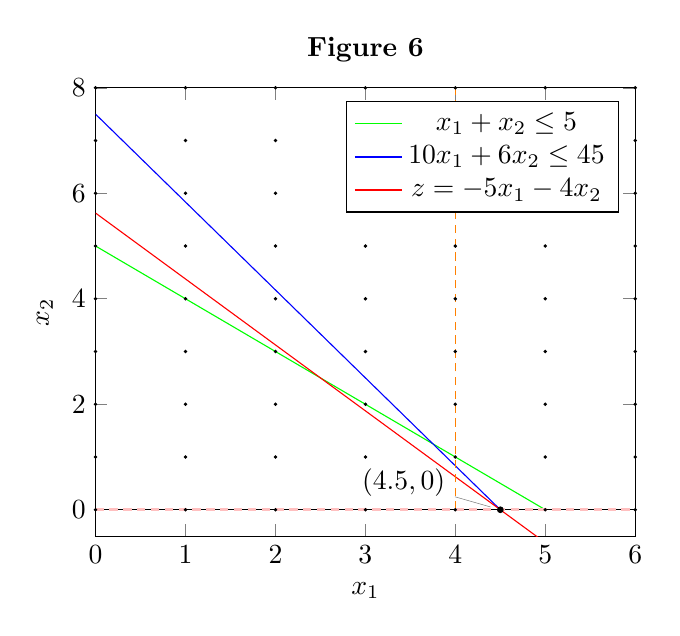
\begin{tikzpicture}
      \begin{axis}[
            xlabel=$x_1$,
            ylabel=$x_2$,
            title =\textbf{Figure 6},
            ymin=-0.5, ymax=8,
            xmin=0, xmax=6,
            legend pos=north east
         ]
         \addplot[color=green,name path=A,domain=0:5]{(5-x};
         \addplot[color=blue,name path=B, domain=0:4.5]{(45-10*x)/6};
         \addplot[color=red,name path=D, domain=0:85]{(22.5-5*x)/4};
         \addplot[name path=C, domain=0:8 , transparent]{1};
         \addplot[name path=E, domain=0:8]{0};
         \addplot +[mark=none , color=orange ] coordinates {(4,0) (4, 8)};
         \addplot +[mark=none , color=pink, line width=0.35mm] coordinates {(0,0) (8, 0)};
         
         \addplot[mark=* , mark size = 1,color=black] coordinates {(4.5,0)} node[pin=175:{$(4.5,0)$}]{};
         
         \foreach \a in {0,...,8}
         \foreach \b in {0,...,8}
         {\addplot[mark=* ,mark size = 0.4] coordinates {(\a,\b)};}
                           
         \addlegendentry{$x_1 +x_2 \leq 5$}
         \addlegendentry{$10x_1 +6x_2 \leq 45$}
         \addlegendentry{$z= -5x_1-4x_2$}
                     
      \end{axis}
   \end{tikzpicture}
   \\
   Le point trouvé est $(4.5,0)$ avec un z de valeur -22.5\\
   Le point n'est pas entier donc nous introduisons $x_1\leq4$ et $x_1\geq5$ \\
   \textbf{$x_1\geq 5 $ n'est pas réalisable}
\end{center}

\pagebreak

\begin{equation*}
   \begin{aligned}
      & \underset{}{\text{minimiser}}
      & & z= -5x_1-4x_2 \\
      & \text{sujet à}
      & & x_1 +x_2 \leq 5\\
        &   &   & 10x_1 +6x_2 \leq 45               \\
        &   &   & x_2 \leq 1                        \\
        &   &   & x_2 \leq 3                        \\
        &   &   & x_2 \leq 0            \\
        &   &   & x_1 \geq 4                 \\ 
      &   &   & x_1 \leq 4                  \\
        &   &   & x_1, x_2 \ge 0 \text{ et entier } 
   \end{aligned}
\end{equation*}
\begin{center}
   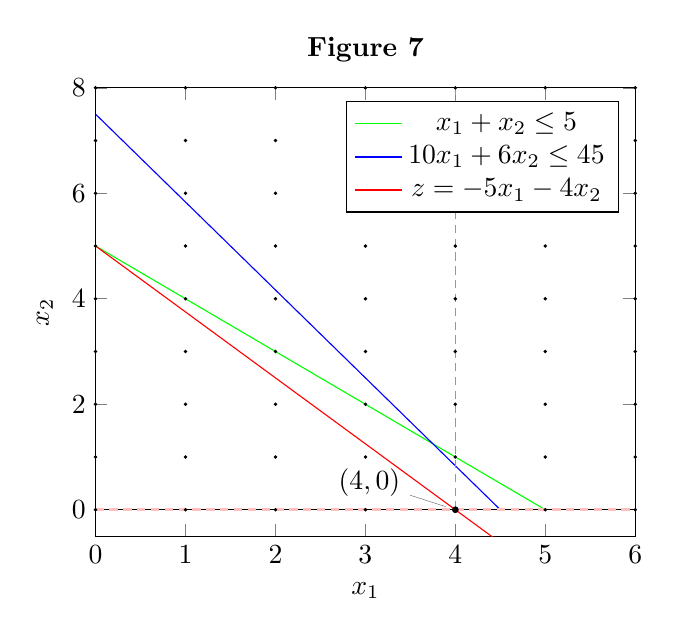
\begin{tikzpicture}
      \begin{axis}[
            xlabel=$x_1$,
            ylabel=$x_2$,
            title =\textbf{Figure 7},
            ymin=-0.5, ymax=8,
            xmin=0, xmax=6,
            legend pos=north east
         ]
         \addplot[color=green,name path=A,domain=0:5]{(5-x};
         \addplot[color=blue,name path=B, domain=0:4.5]{(45-10*x)/6};
         \addplot[color=red,name path=D, domain=0:85]{(20-5*x)/4};
         \addplot[name path=C, domain=0:8 , transparent]{1};
         \addplot[name path=E, domain=0:8]{0};
         \addplot +[mark=none , color=orange ] coordinates {(4,0) (4, 8)};
         \addplot +[mark=none , color=pink, line width=0.35mm] coordinates {(0,0) (8, 0)};
         
         \addplot[mark=* , mark size = 1,color=black] coordinates {(4,0)} node[pin=175:{$(4,0)$}]{};
         
         \foreach \a in {0,...,8}
         \foreach \b in {0,...,8}
         {\addplot[mark=* ,mark size = 0.4] coordinates {(\a,\b)};}
                           
         \addlegendentry{$x_1 +x_2 \leq 5$}
         \addlegendentry{$10x_1 +6x_2 \leq 45$}
         \addlegendentry{$z= -5x_1-4x_2$}
                     
      \end{axis}
   \end{tikzpicture}
   \\
   Le point trouvé est $(4,0)$ avec un z de valeur -20\\
   Le point est un entier donc nous ne branchons pas
\end{center}
\pagebreak
\subsection*{Analyse}
On peut voir que la solution entière la plus optimale est (3,2) avec $z = -23$\\
Les autres solutions entières étant (3,1) et (4,0) avec un z de valeur -19 et -20 respectivement 
\linebreak
\begin{center}
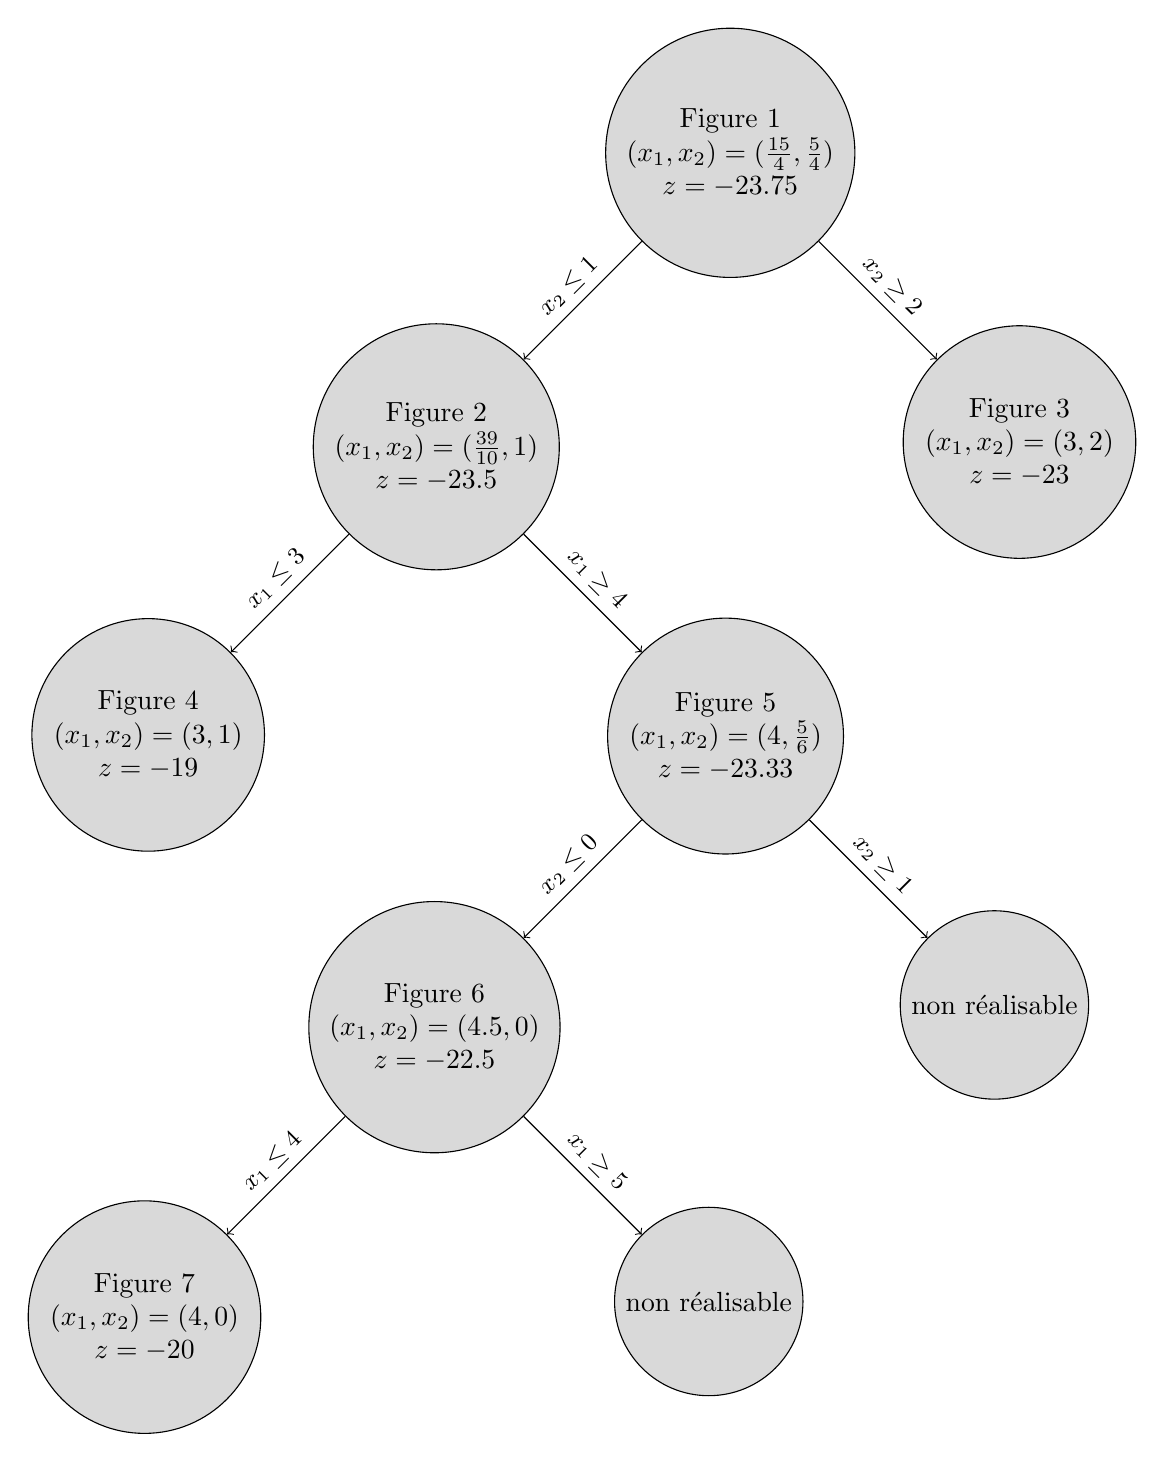
\begin{tikzpicture}[
node distance = 15mm and 15mm,
     V/.style = {circle, draw, fill=gray!30},
every edge quotes/.style = { font=\small, sloped}
                    ]
    \begin{scope}[nodes=V]
\node (1)  [align=center] {Figure 1 \\ $(x_1,x_2)=(\frac{15}{4},\frac{5}{4})$ \\ $z=-23.75$};
\node (2) [below left=of 1 , align=center]   {Figure 2 \\ $(x_1,x_2)=(\frac{39}{10},1)$ \\ $z=-23.5$ };
\node (3) [below right=of 1, align=center]  {Figure 3 \\ $(x_1,x_2)=(3,2)$ \\ $z=-23$};
\node (4) [below left=of 2,align=center]   {Figure 4 \\ $(x_1,x_2)=(3,1)$ \\ $z=-19$};
\node (5) [below right=of 2,align = center] {Figure 5 \\ $(x_1,x_2)=(4,\frac{5}{6})$ \\ $z=-23.33$};
\node (6) [below left=of 5, align=center]   {Figure 6 \\  $(x_1,x_2)=(4.5,0)$ \\ $z=-22.5$};
\node (7) [below right=of 5] {non réalisable};
\node (8) [below left=of 6, align=center]   {Figure 7 \\  $(x_1,x_2)=(4,0)$ \\ $z=-20$};
\node (9) [below right=of 6] {non réalisable};




    \end{scope}
\draw   (1)  edge[->,"$x_2\leq 1$",above] (2)
        (1)  edge[->,"$x_2 \geq 2$",above] (3)

        (2)  edge[->,"$x_1 \leq 3$",above] (4) 
        (2)  edge[->,"$x_1 \geq 4$",above] (5)

        (5)  edge[->,"$x_2 \leq 0$",above] (6) 
        (5)  edge[->,"$x_2 \geq 1$",above] (7)

        (6)  edge[->,"$x_1 \leq 4$",above] (8) 
        (6)  edge[->,"$x_1 \geq 5$",above] (9);
    \end{tikzpicture}
\end{center}


\end{document}
